\documentclass[11pt, letterpaper, includehead]{article}

%%%%%%%%%%%%%%%%%%%%% Pre-document %%%%%%%%%%%%%%%%%%%%%
\usepackage{fancyhdr}  % Allow for headers
\usepackage{graphicx}  % Allow for figures 
\usepackage{float}     % Allow for figure inserted in specified location
\usepackage{amsmath}   % Allow for aligned math
\usepackage{array}     % Allow for cell width manipulation
\usepackage{nicematrix}
\usepackage{multicol}

\setlength{\parindent}{0pt} % Remove auto paragraph indents

% Get rid of those big ass margins
\usepackage[margin=1in]{geometry}

% Table cell formatting
\setlength{\arrayrulewidth}{0.25mm}
\setlength{\tabcolsep}{11pt}
\renewcommand{\arraystretch}{1.2}

\begin{document}

%%%%%%%%%%%%%%%%%%%%% Title Page %%%%%%%%%%%%%%%%%%%%%
\begin{titlepage}
  \begin{center}
    \Huge{\textbf{Lab 5}}\\
    \Huge{Forces and Acceleration}
    \vfill
    \begin{figure}[H] % H makes the figure insert at the position in the document
      \centering 
      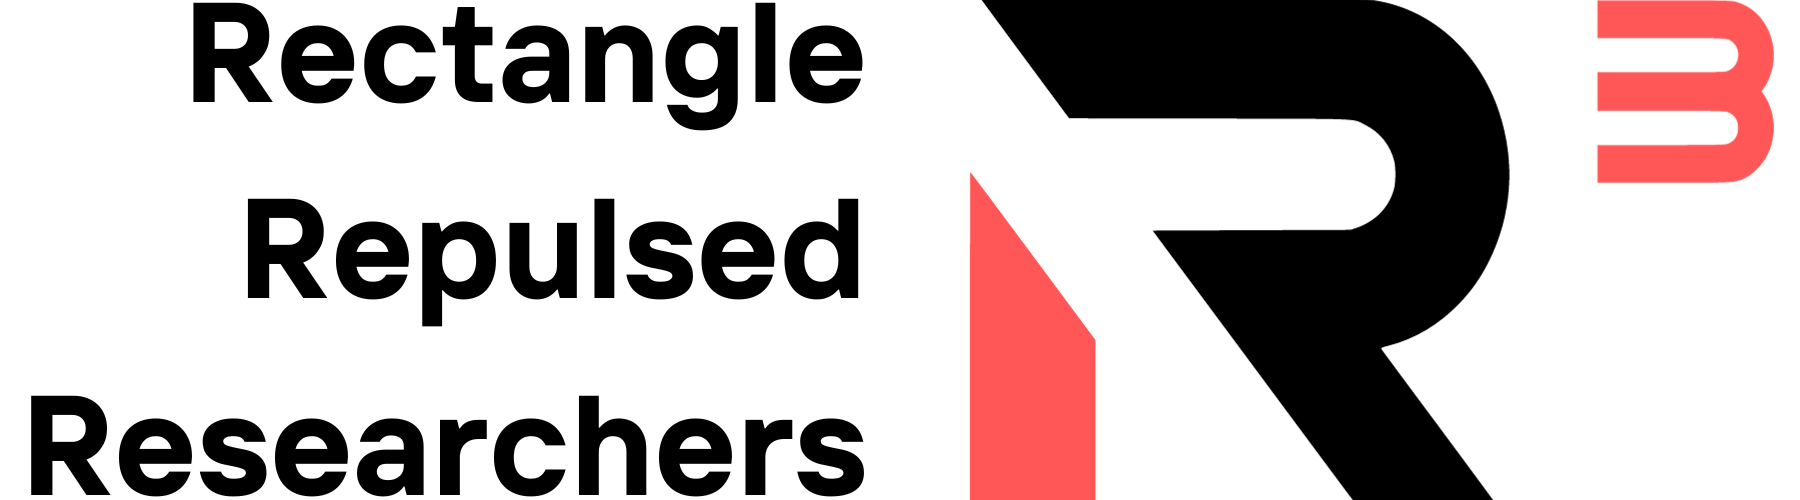
\includegraphics[width=6cm]{../logo.png}
    \end{figure}
    \large{\textbf{your name here}}\\
    \large{Julian Barossi, Liam Gilligan, Stephanie L'Heureux}\\
    \vspace{0.5cm}
    \normalsize
    \today
  \end{center}
\end{titlepage}

%%%%%%%%%%%%%%%%%%%%% TABLE OF CONTENTS %%%%%%%%%%%%%%%%%%%%%
\tableofcontents
\pagebreak % Move to next page

% Add a nice fancy header
\pagestyle{fancy}
\fancyhead{}
\fancyhead[C]{\textbf{Lab 5:} Forces and Acceleration}

\section{Level track} % 1
\subsection{Free body diagram} % 1.1
\subsection{Predicted acceleration of the system} % 1.2
\subsection{Predicted time} % 1.3
\subsection{Experimental time} % 1.4
\subsection{Analysis} % 1.5
\subsection{Tension} % 1.6
\section{Sloping air track I} % 2
\subsection{Free body diagram}
\subsection{Predicted acceleration of the system}
\subsection{Predicted time}
\subsection{Experimental time}
\subsection{Analysis}
\section{Sloping air track II} % 3
\subsection{Free body diagram}
\subsection{Predicted acceleration of the system}
\subsubsection{Calculate theta}


\begin{center} 
  \begin{tabular}{|  m{8cm} | m{2cm} | m{2cm} | } 
    \hline
    \textbf{Quantity} & \boldmath{$cm$} & \boldmath{$m$}\\ 
    \hline
    Block height & 4.50 & 0.05 \\ 
    \hline
    Track length & 98.60 & 0.99 \\ 
    \hline
    $\theta$ (degrees) & 2.62 & 2.62 \\ 
    \hline
  \end{tabular} 
\end{center}

$$\sum F = m_1 a$$
$$m_1 g - T = m_1 a$$
$$m_1 g - m_1 a = T$$

$$\sum F = m_2 a$$
$$T - m_2 g \sin(\theta) = m_2 a$$
$$T = m_2 g \sin(\theta) + m_2 a$$
$$m_1 g - m_1 a = m_2 g \sin(\theta) + m_2 a$$
$$m_1 g - m_2 g \sin(\theta) = m_2 a + m_1 a$$
$$m_1 g - m_2 g \sin(\theta) = a(m_1 + m_2)$$
$$a = \frac{m_1 g - m_2 g \sin(\theta)}{m_1 + m_2}$$
$$a = \frac{g(m_1  - m_2  \sin(\theta))}{m_1 + m_2}$$
$$a = \frac{(9.8m/s^2)(0.015 kg - 0.149kg \sin(2.612^{\circ}))}{0.015 kg + 0.149kg}$$
$$a = 0.490582058...m/s^2 \approx 0.491m/s^2$$
$$\boxed{a = 0.491m/s^2}$$

\subsection{Predicted time}
$$\Delta x = v_ot + \frac{1}{2}at^2$$
$$\Delta x = (0m/s)t + \frac{1}{2}at^2$$
$$\Delta x = \frac{1}{2}at^2$$
$$t = \sqrt{\frac{2\Delta x}{a}}$$
$$t = \sqrt{\frac{2 \cdot 0.908 m}{0.491m/s^2}}$$
$$t = 1.923167787...s \approx 1.92s$$
$$\boxed{t = 1.92s}$$
\subsection{Experimental time}
\begin{center} 
  \begin{tabular}{|  m{5cm} | m{5cm} | } 
    \hline
    \textbf{Trial} & \textbf{Time (s)} \\ 
    \hline
    1 & 1.88 \\ 
    \hline
    2 & 1.88 \\ 
    \hline
    3 & 1.92 \\ 
    \hline
    4 & 2.06 \\ 
    \hline
    5 & 1.97 \\ 
    \hline
    6 & 1.85 \\ 
    \hline
    7 & 1.93 \\ 
    \hline
    8 & 1.91 \\ 
    \hline
    9 & 2.03 \\ 
    \hline
    10 & 2.01 \\ 
    \hline
    \hline
    \boldmath{$t_{expt}$} & 1.94 \\ 
    \hline
    \boldmath{$\sigma_t$} & 0.07 \\ 
    \hline
    \boldmath{$SE$} & 0.02 \\ 
    \hline
  \end{tabular} 
\end{center}

\subsection{Analysis}
\subsection{Tension}

\end{document}
